\section{Planning Cost Functions}


\subsection{Pixel-Distance based Cost}
A convenient way to define a robot task is by choosing one or more pixels in the robot's camera view and choosing a destination where each pixel should be moved. For example, the user might select a pixel on an object and ask the robot to move it 10 cm to the left. Formally, the user specifies $P$ source pixel locations $\pixel_0^{(1)}, \dots, \pixel_0^{(P)}$ in the initial image $I_0$, and $P$ goal locations $\goal^{(1)}, \dots, \goal^{(P)}$. The source and goal pixel locations are denoted by the coordinates $(x_d^{(i)}, y_d^{(i)})$ and $(x_g^{(i)}, y_g^{(i)})$. Given a goal, the robot plans for a sequence of actions $\action_{1:T}$ over $T$ time steps, where $T$ is the planning horizon. For this type of task definition the problem is formulated as the minimization of a cost function $c$ which depends on the predicted pixel positions $d_t^{(j)}$. The planner makes use of a learned model that predicts a distribution over the pixel position by internally predicting pixel transformations. Given a distribution over pixel positions $P_{t_0, d^{(i)}}\in\mathbb{R}^{H\times W}$ at time $t = 0$, the model predicts distributions over its positions $P_{t, d^{(i)}}$ at time $t \in \{ 1, \dots, T \}$. The optimizer then finds the action sequence $a_{t_0:T}$ for which the sum of the costs $c_t$ over the time steps is minimal. $c_t$ is defined as the expected euclidean distance between to the goal point $g^{(i)}$ (which is straight-forward to calculate from $P_{t, d^{(i)}}$ and $g^{(i)}$).

The expected distance to the goal provides smoother planning objective that makes used of the uncertainty estimates of the predictor enabling complex, longer-horizon tasks. This cost function encourages the movement of the designated objects in the right direction for each step of the execution, regardless of whether the $\goal$ position can be reached within $T$ time steps. For multi-objective tasks with multiple designated pixels $d^{(i)}$ the costs are summed to together (and optionally weighting them according to a scheme discussed in \autoref{subsec:reg_cost}).  

\subsection{Registration-based Cost}
\label{subsec:reg_cost}
For the type of cost function introduced in the previous section it necessary to know the initial locations $\pixel_0^{(1)}, \dots, \pixel_0^{(P)}$ at each timesteps. However when the tobot interacts with an object, the position of that object may change in unexpected ways, and therefore it is crucial that the system can update its belief of where the target object is. Prior work on visual MPC lacked this capability. To enable the agent to ``keep retrying" indefinitely until the task is accomplished we propose to use an image-to-image registration approach to find the target object in the current frame. 
We show that this tracking capability can be learned completely unsupervised from the data collected by the robot autonomously. As one might expect the self-supervised tracking approach works better for images that are closer to each other and sometimes fails when the entities in the image are too far apart. To increase accuracy and robustness in addition to the starting image our method can register to a goal-image. The goal image is optional and can be provided by a human or through demonstration.

\subsubsection{Test time procedure}

We will first describe the architecture at test time (see Figure~\ref{fig:registration_arch}). The start and goal images $I_0$ and $I_g$ are passed into the registration network $R$ which returns flow maps:
\begin{align}
    \hat{F}_{0 \leftarrow t} = R(I_t, I_0) &&
    \hat{F}_{g \leftarrow t} = R(I_t, I_g)
\end{align}

The flow maps warp the image of the current time step to the start image $I_0$, and $\hat{F}_{g \leftarrow t}$ warps from $I_t$ to $I_g$ (see Figure \ref{fig:reg_single} for an illustration):
\begin{align}
    \hat{I}_0 = \hat{F}_{0 \leftarrow t} \diamond  I_t &&
    \hat{I}_g = \hat{F}_{g \leftarrow t} \diamond  I_t 
\end{align}
Here, $\diamond$ denote a bilinear sampling operator which interpolates a position in an image bilinearly with respect to a location $(x,y)$ in the image. In addition to start and goal images, the user needs to specify one or several designated pixel positions $d_0$ in the start image and the corresponding pixels locations $d_g$ in the goal image (the goal image is optional) to define the task. While the registration network is trained to perform a global registration between the images, we only evaluate it at the points $d_0$ and $d_g$ chosen by the user. This results in a cost function that ignores distractors.  $R$ takes in a pair of images and outputs a flow-map warping points in one to the other. Thus, for a current image $I_t$, $\hat{F}_{0 \leftarrow t}$ puts it in correspondence with $I_0$, and $\hat{F}_{g \leftarrow t}$ puts it in correspondence with $I_g$. The registration network is then used to find the pixel locations corresponding to $d_0$ and $d_g$ in the current frame: 
\begin{align}
    \hat{d}_{0,t} = d_0 + \hat{F}_{0 \leftarrow t}(d_0) &&
    \hat{d}_{g,t} = d_g + \hat{F}_{g \leftarrow t}(d_g)
\end{align}
  
%%SL.06.12: I wonder if we can defer all the discussion of designated pixels to some other section. We can use registration even without designated pixels, and I think the technical sections would be easier to follow if we first just describe registration by itself, and then later talk about how it can actually be combined with designated pixels, which serve both to define the goal and to focus the cost function on the objects that actually matter.

\begin{figure}[t!]
    \centering
    \begin{subfigure}[b]{0.35\columnwidth}
        \centering
        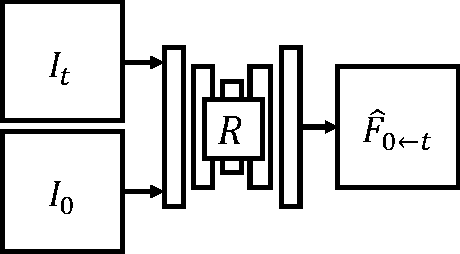
\includegraphics[width=\columnwidth]{images_rfr/registration_test_start.pdf}\vspace{2.5mm}
        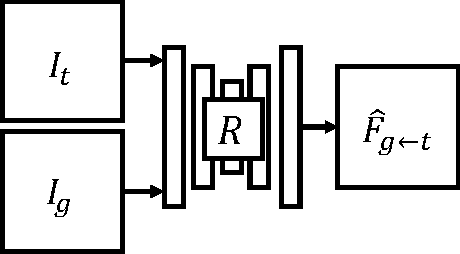
\includegraphics[width=\columnwidth]{images_rfr/registration_test_goal.pdf}
        \caption{\small{Testing usage.}}
    \end{subfigure}
    \quad \quad
    \begin{subfigure}[b]{0.55\columnwidth}
        \centering
        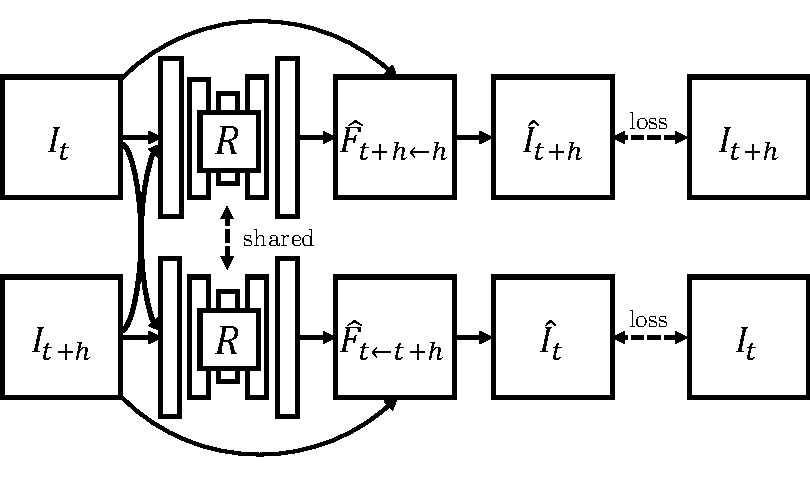
\includegraphics[width=\columnwidth,trim={0 3mm 0 3mm},clip]{images_rfr/registration_train.pdf}
        \caption{\small{Training usage.}}
        \label{fig:discrete}
    \end{subfigure}
    \vspace{-1mm}
    \caption{\small{(a) At test time the registration network registers the current image $I_t$ to the start image $I_0$ (top) and goal image $I_g$ (bottom), inferring the flow-fields $\hat{F}_{0 \leftarrow t}$ and $\hat{F}_{g \leftarrow t}$. (b) The registration network is trained by warping images from randomly selected timesteps along a trajectory to each other.
    }}
    \label{fig:registration_arch}
\end{figure}

\begin{figure*}
    \centering
    \vspace{-0.1in}
    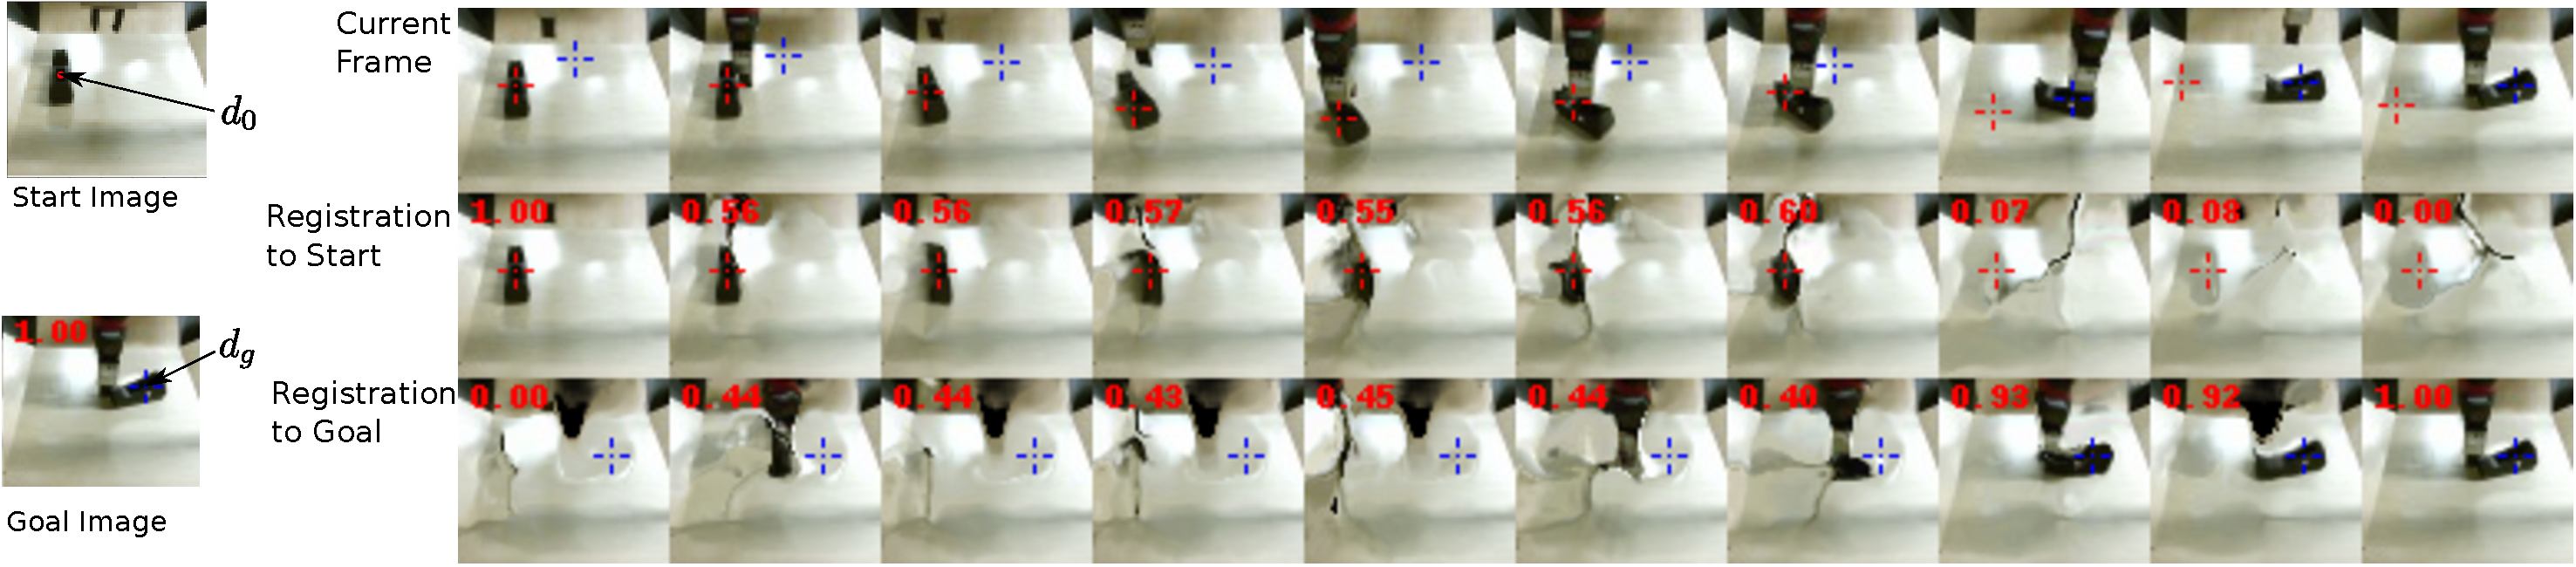
\includegraphics[width=1\linewidth]{images_rfr/registration_overtime.pdf}
    \caption{\small{Outputs of registration network. The first row shows images from a trajectory executed by the robot, the second shows each image warped to the initial image via registration, and the third shows the same for the goal image. A successful registration in this visualization would result in images that closely resemble the start (or goal). In these images, the locations where the designated pixel of the start image $d_0$ and the goal image $d_g$ are found is marked with red and blue crosses, respectively. It can be seen that, for the registration to the start image (red cross) the object is tracked for the first 7 frames, while the registration to the goal image (blue cross) succeeds for the last 3 time steps. The numbers in red indicate the trade off factors $\lambda$ between the views and are used as weighting factors for the planning cost.}}
    \label{fig:tracking_overtime}
    \vspace{-0.2in}
\end{figure*}

\autoref{fig:tracking_overtime} visualizes the tracking results during a pushing task. On the left we show the start image and goal image provided by the user at the beginning of the trajectory. The first row shows the video, with the estimated location of $d_0$ marked in red and the estimated location of $d_g$ marked in blue. In this example, registration succeeds with respect to the first image succeeds for the first 7 steps but fails after that. However registration with respect to the goal image succeeds for the last 3 steps. Thus, there is enough information at each time step to determine the cost, which we discuss in detail in the next section.


\subsubsection{Train time procedure}
The registration network $R$ is trained to find correspondences between two images by warping one image to the other. The network is trained on the same data as the video-prediction model, but it does not share parameters with it.\footnote{in principle sharing parameters with the video-prediction model might be beneficial, however this is left for future work} This approach is similar to the optic flow method proposed by \cite{meister2017unflow}. However, unlike this prior work, our method computes registrations for frames that might be many time steps apart, and the goal is not to extract optic flow, but rather to determine correspondences between potential highly distinct images. For training, two images are sampled at random times steps $t$ and $t+h$ along the trajectory and the images are warped to each other in both directions. 
\begin{align}
     \hat{I}_{t} = \hat{F}_{t \leftarrow t +h} \diamond  I_{t+h} &&
     \hat{I}_{t+h} = \hat{F}_{t+h \leftarrow t} \diamond  I_{t}
\end{align}
The network, which outputs $\hat{F}_{t \leftarrow t +h}$ and $\hat{F}_{t+h \leftarrow t}$ (see Figure~\ref{fig:registration_arch}), is trained to minimize the photometric distance between $\hat{I}_t$ and $I_t$ and $\hat{I}_{t+h}$ and $I_{t+h}$, in addition to a smoothness regularizer that penalizes abrupt changes in the outputted flow-field. The details of this loss function follow prior work \cite{meister2017unflow}. We found that gradually increasing the temporal distance $h$ between the images during training yielded better final accuracy, as it created a curriculum for the model. The network $R$ is implemented as a fully convolutional network which takes in as input the two images stacked together along the channel dimension. We use three convolutional layers each followed by a bilinear downsampling operation followed by three layers of convolution each followed by a bilinear upsampling operation (all convolutions use stride 1). In this way we avoid artifacts due to strided convolutions and deconvolutions.


\subsection{Classifier-based Cost}
\label{subsec:class_cost}
An alternative way to define the cost function is with a goal classifier. This type of cost function is particularly well-suited for tasks that can be completed in multiple ways. For example, for a task of rearranging a pair objects into relative positions, i.e. pushing the first object to the left of the second object, the absolute positions of the objects do not matter. A classifier-based cost function allows the planner to discover any of the possible goal states.

\newcommand{\task}{\mathcal{T}}
\newcommand{\data}{\mathcal{D}}
\newcommand{\obs}{\mathbf{o}}
\newcommand{\out}{y}
\newcommand{\posdata}{\data^+}
\newcommand{\testdata}{\data^\text{test}}
\newcommand{\loss}{\mathcal{L}}

Formally, we consider a goal classifier $\hat{\out} = f(\obs)$, where $\obs$ denotes the image observation, and $\hat{\out} \in [0,1]$ indicates the predicted probability of the observation being of a successful outcome of the task. Our objective is to infer a classifier for a new task $\task_j$ from a few positive examples of success, which are easy for a user to provide and encode the minimal information needed to convey a task. In other words, given a dataset $\posdata_j$ of $K$ examples of successful end states for a new task $\task_j$: $\data_j:=\{(\obs_k, 1) | k = 1...K\}_j$, our goal is to infer a classifier for task $\task_j$.

\subsection{Which cost function is best?}
adsf


\subsubsection{Meta-Learning for Few-Shot Goal Inference}

To solve the above problem, we propose learning a few-shot classifier that can infer the goal of a new task from a small set of goal examples, allowing the user to define a task from goal images alone.

To train the few-shot classifier, we build upon model-agnostic meta-learning (MAML)~\cite{maml}, which learns initial parameters $\theta$ for model $f$ that can efficiently adapt to a new task with one or a few steps of gradient descent. \cite{caml} proposed an extension of MAML, referred to as concept acquisition through meta-learning (CAML), for learning new concepts from positive examples alone. We apply CAML to the setting of acquiring goal classifiers from positive examples.

\subsubsection{Test time procedure}
At test time, the user provides a dataset $\posdata_j$ of $K$ examples of successful end states for a new task $\task_j$: $\data_j:=\{(\obs_k, 1) | k = 1...K\}_j$, which are then used to infer a task-specific goal classifier $C_j$. In particular, the meta-learned parameters $\theta$ are updated through gradient descent to adapt to task $\task_j$:

$$
C_j(\obs)
= f(\obs; \theta_j')
= f\big(\obs; \theta-\alpha \nabla_\theta \!\!\! \sum_{(\obs_n, \out_n)\in \posdata_j} \loss (\out_n, f(\obs_n; \theta)\big)
$$

where $\loss$ is the cross-entropy loss function, $\alpha$ is the step size, and $\theta'$ denotes the parameters updated through gradient descent on task $\task_j$.

During planning, the learned classifier $C_j$ takes as input an image generated by the video-prediction model and outputs the predicted probability of the goal being achieved for the task. Concretely, the cost is defined as the negative of the classifier prediction.


\subsubsection{Train time procedure}
During meta-training, we explicitly train for the ability to infer goal classifiers for the set of training tasks, $\{ \task_i \}$. We assume a small dataset $\data_i$ for each task $\task_i$, consisting of both positive and negative examples: $\data_i:= \{(\obs_n,\out_n) | n=1...N \}_i$. To learn the initial parameters $\theta$, we optimize the following objective:

$$
\min_\theta \sum_i \sum_{(\obs_n, y_n) \in \testdata_i} \loss(\out_n, f(\obs_n; \theta_i')) 
$$

We optimize this objective using Adam~\cite{ADAM} on the initial parameters $\theta$. In our experiments, our classifier is represented by a convolutional neural network, consisting of three convolutional layers, each followed by layer normalization and a ReLU non-linearity. After the final convolutional layer, a spatial soft-argmax operation extracts spatial feature points, which are then passed through fully-connected layers.